\documentclass[10pt]{article}

%/ Use case: language and spell checking
\usepackage[utf8]{inputenc}
\usepackage[dutch]{babel}
%/ Use case: uppercase headers
\usepackage{titlecaps}
\usepackage{sectsty}
%/ Use case: text formatting
\usepackage{url}
\usepackage[outputdir=tmp]{minted}
\usepackage[colorlinks=true, allcolors=teal]{hyperref}
\usepackage{textcomp}
\usepackage{amsmath}
%/ Use case: images
\usepackage{graphicx}
\usepackage[export]{adjustbox}
\usepackage[font=small,labelfont=bf]{caption}
%/ Use case: tables
\usepackage{booktabs}
\usepackage[flushleft]{threeparttable}
\usepackage{pgfplots}
\usepackage{pgfplotstable}

\graphicspath{ {./img/} }

\pgfplotsset{compat=1.18}

\allsectionsfont{\mdseries\scshape}

\title{\titlecap{\scshape Project Robotica}\normalfont}
\author{Wessel Tip $<$contact@wessel.gg$>$ (\url{https://wessel.gg/}) \\
Technische Informatica \\
Hoogeschool Inholland Alkmaar \\
 Jaar 2, Semester 2 (Jan. 2024 - Jun. 2024)
}

\begin{document}

\maketitle

% \begin{abstract}
% In dit verslag zal besproken worden waarom er is gekozen om een RESTful API
% te maken voor het project Robotica.

% De toegankelijkheid en schaalbaarheid van de API-architecturen REST, SOAP,
% GraphQL en gRPC zullen worden vergeleken om uiteindelijk op de conclusie te
% komen waarom REST gebruikt word.
% \end{abstract}

\tableofcontents
\newpage

\section{Inleiding}
\label{sec:inleiding}

In de moderne softwareontwikkeling spelen API's (Application Programming Interfaces)
een belangrijke rol. Ze vormen de brug tussen verschillende softwarecomponenten
en zorgen voor een gestructureerde manier om gegevens uit te wisselen.\cite{masse2011}

In het Robotica-project, waarbij voor mijn persoonlijke bijdrage de communicatie
tussen de gebruiker en de robot centraal staat,
is de keuze van een geschikte API-architectuur van groot belang.

De API moet eenvoudig te implementeren en te onderhouden zijn.
Dit verslag zal vier verschillende API architecturen bespreken en vergelijken
om uiteindelijk tot de conclusie te komen voor welk architectuur het beste is
voor het project.

\section{Probleemstelling}
\label{sec: Probleemstelling}

\subsection{Probleemanalyse}
\label{ssec:probleemanalyse}

API's (\textit{Application Programming Interfaces}) zijn onmisbare componenten in moderne
software. Door middel van een API in combinatie met een set van afspraken
(een \textit{protocol}) is het mogelijk meerdere softwarecomponenten met elkaar
te integreren. Deze API's maken de communicatie tussen verschillende
softwarecomponenten mogelijk.\cite{Souza_2012}

Er zijn over de jaren vele verschillende manieren bedacht voor het ontwerpen
en implementeren van API's, elk met zijn eigen voordelen en nadelen.
\cite{Śliwa_Pańczyk_2021} In dit onderzoek wordt er een vergelijking gesteld
tussen vier verschillende API architecturen (REST, SOAP, GraphQL en gRPC)
om te bepalen welke het meest geschikt is voor het project.

Bij het kiezen van een API architectuur wordt er rekening gehouden met een bepaald
aantal criteria. De API moet ontwikkelt worden zonder dat er externe libraries
gebruikt worden. Dit betekent dat de API vanaf de grond af aan moet worden opgebouwd.

De API moet ook in staat zijn om de communicatie tussen de verschillende componenten
van de robot te ondersteunen. Dit betekent dat de API de communicatie tussen de
gebruiker en de robot moet ondersteunen, en de communicatie tussen de verschillende
robots onderling.

De interface die wordt gepresenteerd aan de eindgebruiker dient alle verzamelde
data te laten zien. Hij zal de mapping en de geplande route moeten presenteren
in een overzichtelijke manier. Ook moet de robot diverse commando's vanuit de
gebruiker kunnen ontvangen om zo de gewenste taken uit te kunnen voeren.

De gekozen API-architectuur moet eenvoudig te onderhouden zijn, met een heldere
en overzichtelijke structuur. De architectuur moet ook felxiebel genoeg zijn
om toevoegingen en aanpassingen te ondersteunen zonder dat de codebase herschreven
moet worden.

De robot vereist een structuele manier om deze gegevens uit te wisselen, en
de optie om meerdere robots tegelijkertijd te besturen.

Een bijkomende eis vanuit de opdrachtgever is dat de software van het beroepsproduct
object-georieënteerd is.

\subsection{Vraagstelling}
De hoofdvraag van dit onderzoek luidt:

\begin{quote}
  "\textit{Welke API architectuur is het beste geschikt voor de specifieke eisen
  van het project, waarbij de communicatie tussen verschillende
  softwarecomponenten, de ondersteuning van gebruikersinteracties, en de
  flexibiliteit en onderhoudbaarheid van de code optimaal zijn?}"
\end{quote}

Om deze hoofdvraag te beantwoorden worden de volgende deelvragen geformuleerd:

Voorafgaand aan het project zijn in \autoref{ssec:probleemanalyse} een aantal
eisen opgesteld, zoals dat de API moet worden opgebouwd zonder het benut van
externe libraries. De volgende deelvraag zal dit beantwoorden:

\begin{quote}
  "\textit{Welke stappen zijn nodig om de API vanaf de grond af aan op te bouwen?}"
\end{quote}

Ook zal er gekeken worden welk architectuur het beste bij het project past. Om
dit te beantwoorden is de volgende deelvraag geformuleerd:

\begin{quote}
  "\textit{Hoe kunnen REST, SOAP, GraphQL, en gRPC worden vergeleken op basis
  van de gestelde criteria?}"
\end{quote}

\section{theoretisch Kader}
\label{sec:theoretisch kader}

\subsection{API-Architecturen}
API's (Application Programming Interfaces) zijn onmisbare componenten in moderne
software. Deze API's maken de communicatie tussen verschillende
softwarecomponenten mogelijk.\cite{Souza_2012}

Er zijn over de jaren vele verschillende manieren bedacht voor het ontwerpen
en implementeren van API's, elk met zijn eigen voordelen en nadelen.
\cite{Śliwa_Pańczyk_2021}

Dit hoofdstuk zal vier van de meest gebruikte API architecturen bespreken.

\subsection{RESTful (Representational State Transfer)}
\label{ssec:rest}
REST is een architectuur dat wordt gebruikt voor het communiceren van gegevens
om netwerkapplicaties te ontwerpen.

Het maakt gebruik van standaard HTTP-methoden (zoals GET, POST, PUT, DELETE)
om gegevens te communiceren tussen clients en servers.\cite{masse2011}

Door de simpiliciteit en het al gebruik maken van de bestaande HTTP protocollen
is REST een populaire keuze voor API's. Dit maakt het ook erg geschikt voor
web gebaseerde applicaties.

\subsubsection{Voordelen van REST}
\label{sssec:voordelen en nadelen van rest}
\begin{enumerate}
  \item \textbf{Eenvoudige structuur} --- gebaseerd op standaard HTTP-methoden
   en JSON
  \item \textbf{Makkelijke implementatie} --- meeste talen ondersteunen de basis
   van webrequests en JSON serialisatie al
  \item \textbf{Schaalbaarheid} --- RESTful API's zijn stateless en kunnen
   eenvoudig horizontaal geschaald worden, echter zal de prestatie wel minder
   zijn dan andere methodes zoals gRPC of GraphQL.\cite{Śliwa_Pańczyk_2021}
\end{enumerate}

\subsubsection{Nadelen van REST}
Echter heeft REST ook zijn nadelen, sommige hiervan zijn:
\begin{enumerate}
  \item \textbf{Overbodig veel data} --- Minder geschikt voor complexere query's
   en datastructuren (over-fetching en under-fetching)
  \item \textbf{Documentatie} --- Geen directe ondersteuning voor documentatie,
   schemas en typecontrole
  \item \textbf{Real-time} --- Doordat de connectie niet levend wordt gehouden nadat
   de aanvrag is afgehandeld is het minder geschikt voor real-time communicatie.
\end{enumerate}

\subsection{SOAP (Simple Object Access Protocol)}
SOAP is een protocol voor uitwisseling van informatie netzoals REST vermeld in
\autoref{ssec:rest}. Echter is SOAP meer complex en minder populair dan REST.

SOAP maakt gebruik van XML voor het sturen van berichten en ondersteunt
in tegenstelling tot REST verschillende transportprotocollen zoals
HTTP en SMTP. SOAP biedt ook robuuste beveiligings- en transactiebeheerfuncties
wat REST niet zo maar heeft.\cite{Śliwa_Pańczyk_2021,w3c}

\subsubsection{Voordelen van SOAP}
\begin{enumerate}
    \item \textbf{Beveiliging} --- Sterke beveiligingsfuncties met behulp van
    WS-Security en ondersteuning voor ACID transacties.
\end{enumerate}

\subsubsection{Nadelen van SOAP}
Net zoals REST heeft SOAP ook zijn nadelen:
\begin{enumerate}
    \item \textbf{Ingewikkeld formaat} --- Complexiteit en overhead door XML-berichten
    \item \textbf{Prestatieproblemen} --- Langzamere prestaties vergeleken met REST
\end{enumerate}

\subsection{GraphQL}
GraphQL is een querytaal voor API's die is ontwikkeld door Facebook in 2012\cite{facebook}.
In tegenstelling tot REST en SOAP, waarbij de server bepaalt welke gegevens
worden geretourneerd, stelt GraphQL clients in staat om een specifieke set data
op te vragen. Ook biedt GraphQL een sterke typecontrole en introspectie aan door
middel van schemas.\cite{Hartig}

\subsubsection{Voordelen van GraphQL}
Voordelen van GraphQL:
\begin{enumerate}
    \item \textbf{Efficiëntie} --- Door de query aard van GraphQL is het
     makkelijk om snel en flexibele bepaalde stukken data aan te vragen.
    \item \textbf{Gegevensbesparing} --- Omdat de gebruiker alleen maar de
     gegevens ontvangt die zij nodig hebben, vermindert dit over-fetching en
     under-fetching waardoor er meer bandbreedte en rekenkracht wordt bespaard.\cite{Hartig}
    \item \textbf{Documentatie} --- Sterke typecontrole en introspectie door het
     gebruik van schemas.
     \item \textbf{compatibiliteit} --- Ook al is het niet gewenst, GraphQL
      is compatibiel met RESTful clients, hierdoor kan de implementatie vrij
      simpel zijn als de kracht van GraphQL niet nodig is.
\end{enumerate}

\subsubsection{Nadelen van GraphQL}
Nadelen van GraphQL:
\begin{enumerate}
    \item \textbf{Intergratie} --- Door de aard van GraphQL is de
     serverimplementatie veel complexer, en daarom ook aangeraden om een library
     te gebruiken.
    \item \textbf{Complexiteit} --- Mogelijkheid van te complexe queries die
     de serverbelasting verhogen
\end{enumerate}

\subsection{gRPC (Google Remote Procedure Call)}
gRPC is een modern RPC-framework dat in 2016 door Google is ontwikkeld. Het maakt
gebruik van HTTP/2 voor transport, Protocol Buffers voor berichtserialisatie en
biedt functies zoals load balancing en monitoring. Door zijn load balancing
functies is gRPC zeer geschikt voor high-performance en real-time communicatie.\cite{google,Śliwa_Pańczyk_2021}

Echter is het wel de moeilijkste methoden om te implementeren en te onderhouden.

\subsubsection{Voordelen van gRPC}
\begin{enumerate}
    \item \textbf{Prestatie} --- Hoge prestaties door het gebruik van protocol
     buffers, berichten zijn tot 30\% kleiner dan JSON.
    \item \textbf{Real-time} --- In tegenstelling tot REST, GraphQL en SOAP
     is gRPC wel geschikt voor real-time communicatie
\end{enumerate}

\subsubsection{Nadelen van gRPC}
\begin{enumerate}
    \item \textbf{Complexiteit} --- Complexer dan alle andere methodes vermeld
     om op te zetten en te debuggen
     \item \textbf{Limitaties} --- Door het vele gebruik van HTTP/2.0 is het niet
      compatibel met oudere web browsers. Ook is er veel minder bekend over gRPC
      dan de andere methodes door zijn relatief nieuwe staat.
\end{enumerate}

\section{Methode}
\label{sec:methode}

\subsection{Welke stappen zijn nodig om de API vanaf de grond af aan op te bouwen?}

\begin{enumerate}
  \item \textbf{Behoeftenanalyse en Specificatie} --- Identificeer de eisen
  voor de API, maak een lijst met de vereiste functies.
  \item \textbf{Architectuurontwerp} --- Definieer de toegestane request types
  (GET, POST, PUT, DELETE) op de benoemde routes en hun verwachte responses.
  \item \textbf{UML ontwerpen} -- Maak een klassendiagram voor de API om de
  structuur van de code te visualiseren.
  \item \textbf{Implementatie} --- Bouw de API volgens de opgegeven eisen en UML
  van punt 1, 2 en 3 op.
  \item \textbf{Testen} --- Ontwikkel unit tests voor alle componenten die
  door de API worden gebruikt. Verwerk vervolgens ieder probleem dat opkomt.
  \item \textbf{Onderhoud} --- Monitor de API na de implementatie,
  pas deze aan op basis van feedback na gebruik. Voeg nieuwe
  functies toe en verbeter de bestaande functies waar nodig, zonder de
  bestaande functionaliteit te breken.
\end{enumerate}

\subsection{Hoe kunnen REST, SOAP, GraphQL, en gRPC worden vergeleken op basis van de gestelde criteria?}

\begin{enumerate}
  \item \textbf{Vergelijkingscriteria} --- Bepaal de
  evaluatiecriteria waarop de architecturen vergeleken zullen worden,
  zoals prestaties, schaalbaarheid en flexibiliteit.
  \item \textbf{Literatuuronderzoek} --- Voer een literatuuronderzoek uit naar de
  kenmerken, voor- en nadelen van REST, SOAP, GraphQL, en gRPC.
  \item \textbf{Theoretische Analyse} --- Analyseer elke API-architectuur op basis
  van de gedefinieerde projectscriteria. Maak een overzicht van de sterke en
  zwakke punten van elke architectuur in de context van het robotica project.
  \item \textbf{Vergelijking} --- Vergelijk de resultaten van de
  analyse. Weeg de voor- en nadelen van elke API-architectuur af tegen de
  specifieke eisen van het project.
  \item \textbf{Conclusie} --- Trek een conclusie over welke API architectuur
  het meest geschikt is voor het project op basis van de vergelijking.
\end{enumerate}

\section{Resultaten}
\label{sec:resultaten}

\subsection{Stappen voor het opbouwen van de API vanaf de grond af aan}
Voor de ontwikkeling van de API zijn de volgende stappen doorlopen:
\begin{enumerate}
  \item \textbf{Behoeftenanalyse en Specificatie} --- De eerste stap was het
  identificeren van de eisen voor de API. De volgende eisen zijn opgesteld na
  aanleiding van de behoeftenanalyse:
  \begin{enumerate}
    \item \textbf{Basisfunctionaliteit}
    \begin{itemize}
      \item Ondersteunen van communicatie tussen de gebruiker en de robot.
      \item Mogelijkheid om de robot te besturen en inzicht te krijgen via een
      webinterface.
    \end{itemize}
    \item \textbf{Technische Specificaties}
    \begin{itemize}
      \item De API moet worden opgebouwd zonder het gebruik van externe libraries.
      \item Gebruik van standaard HTTP-methoden (GET, POST, PUT, DELETE).
      \item Het gebruik van JSON voor gegevensoverdracht.
    \end{itemize}
    \item \textbf{Flexibiliteit en Onderhoudbaarheid}
    \begin{itemize}
      \item Eenvoudige structuur die gemakkelijk te onderhouden is.
      \item Flexibel genoeg om toekomstige toevoegingen en aanpassingen te
      ondersteunen zonder dat de hele codebase herschreven moet worden.
    \end{itemize}
    \item \textbf{Gebruikersinterface}
    \begin{itemize}
      \item Weergave van verzamelde data in een overzichtelijke manier.
      \item Presentatie van de mapping en de geplande route van de robot.
      \item Mogelijkheid om diverse commando’s naar de robot te sturen.
    \end{itemize}
  \end{enumerate}
  \item \textbf{Architectuurontwerp} --- Vervolgens zijn de toegestane request types (GET, POST, PUT, DELETE) gedefinieerd, samen met de benoemde routes en hun verwachte responses. Dit heeft geresulteerd in een gedetailleerd ontwerp van de API-structuur.
  \begin{itemize}
    \item \textbf{GET /api/v1/database/metadata}
    \linebreak Geeft basisinformatie over de database terug.
    \item \textbf{GET /api/v1/database}
    \linebreak \textbf{Query Paramters:}
    \begin{itemize}
      \item ?id=$<$string$>$ --- De UUIDv4 van de gewensde map.
      \item ?name=$<$string$>$ --- De naam van de gewensde map.
      \item ?version=$<$int$>$ --- Het versienummer van de gewensde maps
      \item ?all=$<$bool$>$ -- Laat alle maps zien
    \end{itemize}
    \textbf{Return Body:}
    \begin{minted}[linenos,frame=leftline,framesep=3pt]{json}
    [
      {
        "Id": "<string>",
        "Name": "<string>",
        "Version": "<int>",
        "Objects": "<Array<Array<int, int>>"
        "Date": "<DateTime>"
      }, {...}
    ]
    \end{minted}
    Geeft een lijst van alle maps terug, of een specifieke map op basis van de query parameters.
    \item \textbf{POST /api/v1/database}
    \linebreak \textbf{Request Body:}
    \begin{minted}[linenos,frame=leftline,framesep=3pt]{json}
    {
      "name": "<string>",
      "objects": "<Array<Array<int, int>>>"
    }
    \end{minted}
    \textbf{Return Body:}
    \begin{minted}[linenos,frame=leftline,framesep=3pt]{json}
    {
      "message": "<success|fail>",
      "id": "<string>",
    }
    \end{minted}
    Voegt een nieuwe map toe aan de database.
    \item \textbf{DELETE /api/v1/database}
    \linebreak \textbf{Query Paramters:}
    \begin{itemize}
      \item ?id=$<$string$>$ --- De UUIDv4 van de gewensde map.
      \item ?name=$<$string$>$ --- De naam van de gewensde map.
    \end{itemize}
    Verwijdert de desbetreffende map uit de database.
    \item \textbf{GET /api/v1/database/path}
    \linebreak \textbf{Query Paramters:}
    \begin{itemize}
      \item ?id=$<$string$>$ --- De UUIDv4 van de gewensde route.
    \end{itemize}
    \textbf{Return Body:}
    \begin{minted}[linenos,frame=leftline,framesep=3pt]{json}
    {
      "Id": "<string>",
      "Objects": "<Array<Array<int, int>>"
    }
    \end{minted}
    \item \textbf{POST /api/v1/database/path}
    \linebreak \textbf{Request Body:}
    \begin{minted}[linenos,frame=leftline,framesep=3pt]{json}
    {
      "id": "<string>",
      "objects": "<Array<Array<int, int>>>"
    }
    \end{minted}
    \textbf{Return Body:}
    \begin{minted}[linenos,frame=leftline,framesep=3pt]{json}
    {
      "message": "<success|fail>",
      "id": "<string>",
    }
    \end{minted}
    Voegt een nieuwe geplande route toe aan de database.
    \item \textbf{DELETE /api/v1/database/path}
    \linebreak \textbf{Query Paramters:}
    \begin{itemize}
      \item ?id=$<$string$>$ --- De UUIDv4 van de gewensde route.
    \end{itemize}
    Verwijdert de desbetreffende route uit de database.
    \item \textbf{POST /api/v1/database/path/plan}
    \linebreak \textbf{Request Body:}
    \begin{minted}[linenos,frame=leftline,framesep=3pt]{json}
    {
      "id": "<string>",
      "objects": "<Array<Array<int, int>>>"
    }
    \end{minted}
    \textbf{Return Body:}
    \begin{minted}[linenos,frame=leftline,framesep=3pt]{json}
    {
      "message": "<success|fail>",
      "id": "<string>",
    }
    \end{minted}
    Voegt een nieuwe geplande route toe aan de database.
    \item \textbf{POST /api/v1/roomba/control}
    \linebreak \textbf{Request Body:}
    \begin{minted}[linenos,frame=leftline,framesep=3pt]{json}
    {
      "command": "<string>"
    }
    \end{minted}
    Proxies het commando naar de Roomba.
  \end{itemize}
  \item \textbf{UML ontwerpen} --- Een klassendiagram is gemaakt om de structuur
  van de code te visualiseren. Dit diagram is te vinden in \autoref{fig:uml}.

  De UML is opgedeeld in drie delen: de HTTP server, het data parsen en de endpoints.
  De HTTP server is verantwoordelijk voor het ontvangen van de requests en het
  doorsturen naar de juiste endpoint. Het data parsen zorgt ervoor dat de data
  correct wordt verwerkt en opgeslagen. De endpoints zijn de verschillende routes
  die de API aanbiedt en de bijbehorende acties die worden uitgevoerd.
  \item \textbf{Implementatie} --- De API is opgebouwd volgens de specificaties
  van de vorige stappen. Er is gebruik gemaakt van Csharp zonder externe libraries
  om de functionaliteiten van de API te implementeren.
  \item \textbf{Testen} --- Er zijn unit tests ontwikkeld voor alle componenten
  die door de API worden gebruikt. Eventuele problemen die tijdens het testen naar
  voren kwamen zijn verwerkt en opgelost.
  \item \textbf{Onderhoud} --- Na implementatie is de API gemonitord en aangepast
  op basis van feedback. Nieuwe functies zijn toegevoegd en bestaande functies
  zijn verbeterd waar nodig, zonder de bestaande functionaliteit te breken.
\end{enumerate}

\subsection{Vergelijking van REST, SOAP, GraphQL, en gRPC op basis van gestelde criteria}
De API architecturen zijn vergeleken op basis van de volgende criteria:
prestaties, schaalbaarheid, flexibiliteit, onderhoudbaarheid, en geschiktheid
voor de projectseisen.
Hieronder volgt een samenvatting van de resultaten verzameld in
\autoref{sec:theoretisch kader}.

\subsubsection{REST}
\begin{itemize}
    \item \textbf{Voordelen}: REST heeft een eenvoudige structuur, maakt gebruik van standaard HTTP-methoden en JSON, en is gemakkelijk te implementeren. Het is goed schaalbaar door zijn stateless karakter.
    \item \textbf{Nadelen}: REST kan overbodige data teruggeven, is minder geschikt voor complexe query’s, en biedt geen directe ondersteuning voor documentatie en real-time communicatie.
\end{itemize}

\subsubsection{SOAP}
\begin{itemize}
    \item \textbf{Voordelen}: SOAP biedt beveiligingsfuncties en ondersteuning
    voor ACID-transacties. Het maakt gebruik van XML voor berichtuitwisseling en
    ondersteunt verschillende transportprotocollen.
    \item \textbf{Nadelen}: SOAP heeft een ingewikkeld formaat door de
    XML-berichten, wat resulteert in een hogere complexiteit vergeleken met REST
    waar meerdere typfouten op kunnen treden.
\end{itemize}

\subsubsection{GraphQL}
\begin{itemize}
    \item \textbf{Voordelen}: GraphQL biedt efficiëntie door de mogelijkheid om
    specifieke sets data op te vragen, wat over-fetching en under-fetching
    vermindert. Ook biedt GraphQL type controle door middel van schema's.
    \item \textbf{Nadelen}: De serverimplementatie van GraphQL is complexer,
    waardoor het moeilijker kan zijn om zonder externe libraries te implementeren.
\end{itemize}

\subsubsection{gRPC}
\begin{itemize}
    \item \textbf{Voordelen}: gRPC biedt hoge prestaties door het gebruik van
    Protocol Buffers, en is zeer geschikt voor real-time communicatie door
    HTTP/2. Het biedt ook functies zoals load balancing en monitoring.
    \item \textbf{Nadelen}: gRPC is complexer op te zetten en te debuggen, en
    heeft limitaties door het gebruik van HTTP/2, wat niet compatibel is met
    oudere web browsers. Ook heeft gRPC net als GraphQL een complexe serverimplementatie.
\end{itemize}

\section{Conclusie}
\label{sec:conclusie}

De hoofdvraag van dit onderzoek luidt:

\begin{quote}
  "\textit{Welke API architectuur is het beste geschikt voor de specifieke eisen van het project, waarbij de communicatie tussen verschillende softwarecomponenten, de ondersteuning van gebruikersinteracties, en de flexibiliteit en onderhoudbaarheid van de code optimaal zijn?}"
\end{quote}

Voor het uiteindelijke project zal er gebruik worden gemaakt van \textbf{REST}
als API architectuur. REST is de meest geschikte keuze voor het project, omdat
het voldoet aan de eisen van het project en het ontwikkelen van de API zonder
externe libraries mogelijk maakt. REST is eenvoudig te implementeren en biedt
een breed scala aan mogelijkheden voor communicatie tussen verschillende
componenten.

Om deze hoofdvraag te beantwoorden, zijn de volgende deelvragen geformuleerd:

\begin{quote}
  "\textit{Welke stappen zijn nodig om de API vanaf de grond af aan op te bouwen?}"
\end{quote}

Uit de ontwikkeling van de API blijkt dat er geen nood is voor specifieke
dataselectie, wat GraphQL juist zo sterk maakt. Ook is er geen nood voor
real-time communicatie of authenticatie.

\begin{quote}
  "\textit{Hoe kunnen REST, SOAP, GraphQL, en gRPC worden vergeleken op basis van de gestelde criteria?}"
\end{quote}

Het project stelt een aantal eisen aan de API-architectuur, waaronder het
ontwikkelen zonder externe libraries. Uit \autoref{sec:resultaten} blijkt dat
\textbf{REST} de meest geschikte keuze is op basis van de gestelde criteria.



\section*{Erkenningen}
\label{sec:erkenningen}
De auteur wilt graag de volgende mensen bedanken voor hun contributie bij het schrijven van dit verslag:
\begin{itemize}
  \item[] \makebox[3.2cm]{\textbf{Buurman, W. J.}\hfill} Groepsgenoot
  \item[] \makebox[3.2cm]{\textbf{Slikker, T.}\hfill} Groepsgenoot
  \item[] \makebox[3.2cm]{\textbf{Ottens, N.}\hfill} Opdrachtgever
  \item[] \makebox[3.2cm]{\textbf{Tilmann, K.}\hfill} Opdrachtgever
\end{itemize}

\label{sec:referenties}
\bibliographystyle{IEEEtran}
\bibliography{references}
% \nocite{*}

\newpage
\section{Bijlage}

\subsection*{User Story}
Nadat de robot de ruimte in kaart heeft gebracht en de optimale route bepaald
heeft, moet dit allemaal op een manier toegankelijk worden gesteld aan de
gebruiker.

Dit zal gedaan worden d.m.v. het hosten van een web interface op een aparte
“server PI”. Deze PI zal vervolgens ook een manier van communicatie opstellen
met de roomba PI om vervolgens hun informatie met elkaar te delen.

\subsection*{UML modellen}
\label{ssec:uml model voor de api server}
\begin{figure}[H]
    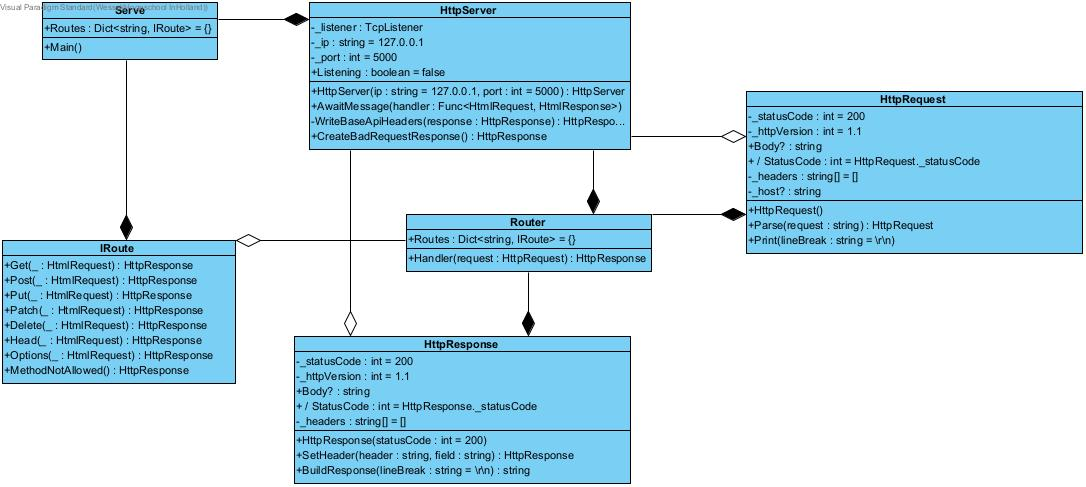
\includegraphics[width=1\textwidth]{uml-v1.jpg}
    \caption{1\textsuperscript{e} versie UML model.}
    \label{fig:umlv1}
\end{figure}

\newpage

\begin{figure}[H]
    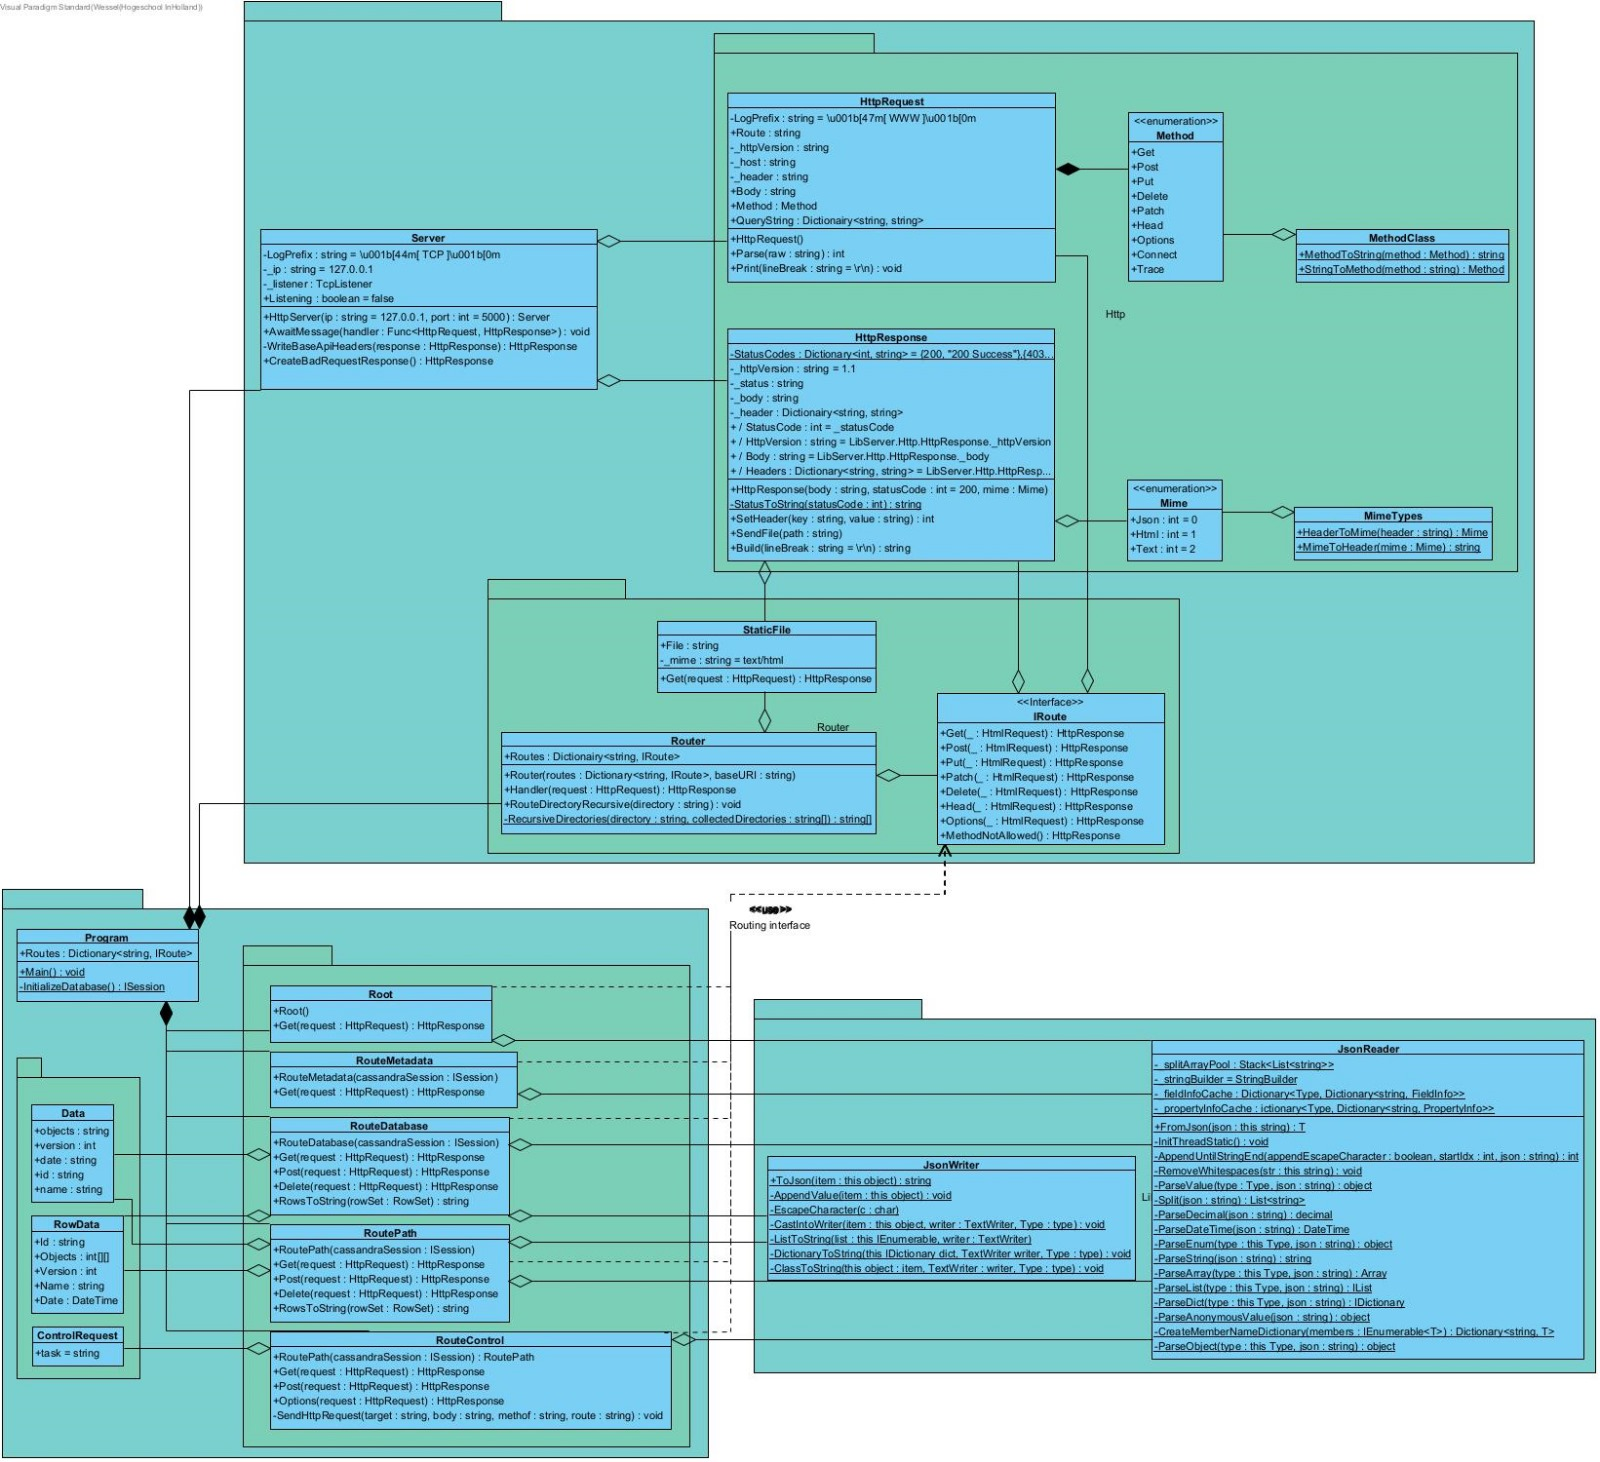
\includegraphics[width=1\textwidth]{uml.jpg}
    \caption{Uiteindelijke versie UML model.}
    \label{fig:uml}
\end{figure}

\newpage


\end{document}
